% !TEX root = BA-Bauer

\subsection{Encoder}
\label{sec:Encoder}
Für die Benutzereingaben sind Taster und vor allem ein Encoder wichtig. Taster ermöglichen eine zeitlich präzise ein Eingabe, wohingegen ein Encoder viele Eingaben in kurzer Zeit ermöglicht. Möchte ein Benutzer eine Aufnahmezeit von 55 Sekunden einstellen, so müsste er 55 mal einen Taster betätigen, mit einem Encoder reichen wenige Umdrehungen dafür aus. In diesem Kapitel wird auf das Funktionsprinzip und die Beschaltung des vewendeten Encoders eingegangen.\\
%Formulierung: Raster bei den Umdrehung ->24
Ein Encoder besteht im einfachsten Sinne aus zwei Schaltern, wie Abbildung \ref{fig:Encoder-Schaltung} zeigt. 
\begin{figure}[h]
	\begin{center}
		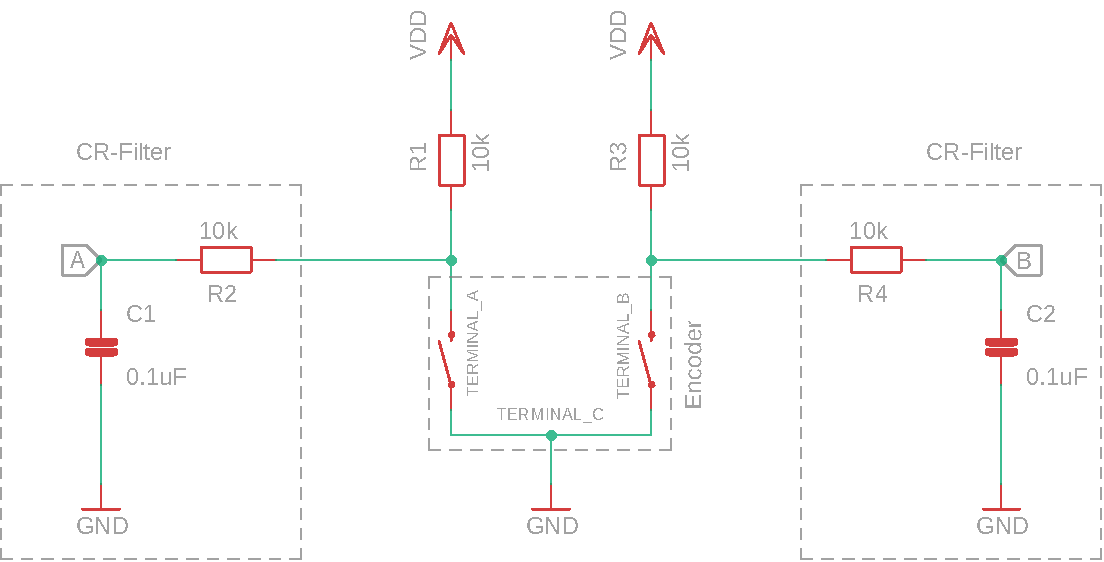
\includegraphics[angle = 0, scale = 1.2]{Encoder-Schaltung-Eagle}
		\caption{Encoder Schaltung \cite{EncoderMN}}
		\label{fig:Encoder-Schaltung}
	\end{center}
\end{figure}
Die Schalter sind auf der einen Seite intern miteinander verbunden (\textit{Terminal C}) und werden auf das 0\,V Potential geschaltet. Die andere Seite der Schalter wird direkt über \textit{Terminal A} und \textit{Terminal B} nach außen geführt. Jeweils ein exerner 10\,k$\Omega$ Pull-Up-Widerstand (R1 und R3) zieht die Ausgänge auf die Betriebsspannug von 5\,V. Ist der Schalter geöffnet, so fließt kein Strom und folglich fällt keine Spannung am Pull-Up-Widerstand ab. Am entsprechenden Terminal können 5\,V gegenüber der Masse gemessen werden. Ist der Schalter geschlossen so fällt die gesamte Spannung am Widerstand ab und am entsprechenden Terminal liegt nun Masse-Potential an. Der Hersteller des Encoders empfiehlt das Beschalten des Encoders mit zwei CR-Tiefpassfiltern um hochfrequente Schaltvorgänge zu filtern. Bei einem Schaltvorgang können die Kontakte des Schalters mechanisch schwingen und dadurch mehrfach hintereinander öffnen und schließen \cite[s. 67]{TechInfo}, wodurch mehfrache Eingaben getätigt werden, obwohl der Encoder nur um einen Schritt gedreht wurde. Die Signale des Encoder werden an Punkt A und B in Abbildung \ref{fig:Encoder-Schaltung} entnommen und über zwei Leiterbahnen zum MCU geführt. %\textbf{Mehr Erklärung??}
\begin{figure}[h]
	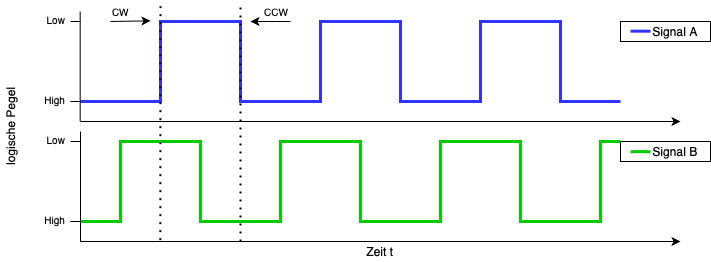
\includegraphics[width=\linewidth]{Encoder-signal}
	\caption{Encoder-Signal bei Drehung im Uhrzeigersinn}
	\label{fig:Encoder-signal}
\end{figure}
Wenn der Encoder gedreht wird schließen und öffnen die internen Schalter versetzt zueinander. Abbildung \ref{fig:Encoder-signal} zeigt die ausgehenden Signale an \textit{Terminal A} und \textit{Terminal B} im zeitlichen Verlauf bei einer gleichmäßigen Rotationsgeschwindigkeit. Durch den versetzten Rhythmus der beiden Schalter kann die Drehrichtung bestimmt werden, indem eines der beiden Signale betrachtet wird, in diesem Beispiel das Signal des \textit{Terminal A}. Ändert sich der Zustand des Signals von \textit{high} auf \textit{low} kann zunächst bestimmt weden, dass eine Drehbewegung stattgefunen hat. Ist nun der Pegel des anderen Signals \textit{high}, so handelt es sich um eine gegen den Uhrzeigersinn drehende Bewegung. Ist das Signal \textit{low}, so handelt es sich um eine mit dem Uhrzeigersinn drehende Bewegung. Die einzelnen Schritte der Schalter können haptisch vom Benutzer wahrgenommen werden. Jeweils an den Stellen an denen sich die Pegel beider $Terminals$ im high-Zustand befinden rastet der Drehregler leicht ein. Dadurch wird sichergestellt, dass sich die Signale des Encoders während der Nichtbenutzung in einem stabilen Zustand befinden. Zudem ergibt sich daraus eine zusätzliche Rückmeldung an den Benutzer während der Eingabe.\\
%-Bewusst gegen Druckknopf entschieden, da zweiter Bestätigungsknopf zur Verwirrung des Benutzers führen kann\\